
%(BEGIN_QUESTION)
% Copyright 2008, Tony R. Kuphaldt, released under the Creative Commons Attribution License (v 1.0)
% This means you may do almost anything with this work of mine, so long as you give me proper credit

Something is wrong with this building alarm system circuit.  The alarm siren refuses to energize even when all windows and doors are opened:

$$\includegraphics[width=15.5cm]{i03197x01.eps}$$

Using your logic probe, you measure a high signal at TP1, a high signal at TP15, and a low signal at TP8 with all windows and doors propped open, and with the key switch in the ``normal'' position.  From this information, identify two possible faults (either one of which could account for the problem and all measured values in this circuit).  Then, choose one of those possible faults and explain why you think it could be to blame.  The circuit elements you identify as possibly faulted can be wires, traces, and connections as well as components.  Be as specific as you can in your answers, identifying both the circuit element and the type of fault.

\begin{itemize}
\item{} Circuit elements that are possibly faulted
\item{1.}
\item{2.} 
\end{itemize}

\begin{itemize}
\item{} Explanation of {\it why} you think one of the above possibilities could be to blame
\end{itemize}

\vfil 

\underbar{file i03197}
\eject
%(END_QUESTION)





%(BEGIN_ANSWER)

This is a graded question -- no answers or hints given!

%(END_ANSWER)





%(BEGIN_NOTES)

A good strategy to begin with when troubleshooting any malfunctioning system is to identify the expected signal states for a properly-functioning system, so that you have a basis for comparison with the measured signal values available to you in the faulted system.  With all doors and windows open, the alarm system activated, and the siren energized, we should expect to see the following states:

\begin{itemize}
\item{} TP1 through TP8 = high
\item{} Voltage between TP10 and TP11 = 120 VAC
\item{} Voltage between TP11 and TP12 = 0 VAC
\end{itemize}

The first point of disagreement between these ideal signal states and our measurements is the signal at TP8: the output of that AND gate should be high with all inputs high, but instead we measure a low state.  Since we know the signal at TP15 is high, either the AND gate is faulted, or it is seeing a low state at TP7, or something is loading its output down so that it cannot achieve a proper high state.

\vskip 10pt

Assuming component faults only (no wires faulted), the following list is a good start.  Note that there may be more circuit elements possibly at fault than what is shown on this list!

\begin{itemize}
\item{} Circuit elements that are possibly faulted
\item{1.} $U_3$ output failed low
\item{2.} $U_4$ output failed low
\item{3.} LED inside SSR failed shorted (causing voltage at TP8 to be too low to be recognized as a high state)
\end{itemize}

%INDEX% Troubleshooting review: electric circuits

%(END_NOTES)


